% !TeX program = xelatex
% New Feature Selection Pipeline -- Gary Wang
% Walkthrough of feature_selection_comparison.py and its outputs

\documentclass[aspectratio=169]{beamer}

\usepackage{graphicx}
\graphicspath{
    {./Figures/}
    {../Meeting_Followup4/Figures/}
    {../../feature_selection/fs_results_v2/png/}
}

\mode<presentation>{
    \usetheme{NordlingLab169}
}

\usepackage[english]{babel}
\let\latinencoding\relax
\usepackage{xltxtra}
\setsansfont{Candara}

\usepackage[yyyymmdd]{datetime}
\renewcommand{\dateseparator}{--}

\usepackage{booktabs}
\usepackage{xcolor}
\usepackage{tikz}
\usetikzlibrary{arrows.meta, positioning, shapes.geometric}

\title[FS Pipeline]{New Feature Selection Pipeline\\\small{LOOCV Benchmark of 28 FS Methods on Tapping Features}}
\author[Gary Wang]{Gary Wang}
\institute[NCKU]{Nordling Lab @
    Dept.\ of Mechanical Engineering\\
    National Cheng Kung University}
\date{\today}

\begin{document}

\setbeamertemplate{background}[NLTitle]
\setbeamertemplate{footline}[NLTitle]
\begin{frame}
    \titlepage
\end{frame}

\setbeamertemplate{background}[NLCC]
\setbeamertemplate{footline}[NLCC]

%%%%%%%%%%%%%%%%%%%%%%%%%%%%%%%%%%%%%%%%%%%%%%%%%%%%%
\begin{frame}
    \frametitle{Motivation}
    \begin{itemize}
        \item Dataset: \textbf{n=53} samples, \textbf{107} numeric tapping features.
        \item Target: MDS-UPDRS finger-tapping rating (0--4 ordinal score).
        \item Goal: identify which feature-selection (FS) method gives the most predictive, compact subset.
        \item Approach: hold the predictor fixed, vary the FS method $\to$ FS effect is isolated.
    \end{itemize}
\end{frame}

%%%%%%%%%%%%%%%%%%%%%%%%%%%%%%%%%%%%%%%%%%%%%%%%%%%%%
\begin{frame}
    \frametitle{Pipeline Overview}
    \centering
    \scalebox{0.78}{%
    \begin{tikzpicture}[
        node distance=0.55cm,
        box/.style={rectangle, rounded corners, draw, thick,
                    minimum width=11cm, minimum height=0.9cm, align=center},
        arr/.style={-Stealth, thick},
    ]
        \node[box, fill=blue!10]   (s1) {\textbf{Stage 1:} Run \textbf{28 FS methods} (filter / embedded / wrapper) on 107 features};
        \node[box, fill=orange!10, below=of s1] (s2) {\textbf{Stage 2:} For each subset $\to$ \textbf{LOOCV} with fixed predictor (MLP-8, tanh, L2)};
        \node[box, fill=green!10,  below=of s2] (s3) {\textbf{Stage 3:} Score with \textbf{4 metrics} (MAE, Spearman, Kappa, Adj.\ Acc.) + 2000-iter bootstrap CIs};
        \node[box, fill=red!10,    below=of s3] (s4) {\textbf{Stage 4:} Rank FS methods by \textbf{Composite} = mean of normalised metrics};
        \node[box, fill=purple!10, below=of s4] (s5) {\textbf{Stage 5:} Among well-performing FS methods, count \textbf{feature inclusion frequency}};
        \draw[arr] (s1) -- (s2);
        \draw[arr] (s2) -- (s3);
        \draw[arr] (s3) -- (s4);
        \draw[arr] (s4) -- (s5);
    \end{tikzpicture}}
\end{frame}

%%%%%%%%%%%%%%%%%%%%%%%%%%%%%%%%%%%%%%%%%%%%%%%%%%%%%
\begin{frame}
    \frametitle{Feature Groups Overview --- Unified Clinical Grouping (107)}
    \scriptsize\centering
    \begin{tabular}{llc}
        \toprule
        \textbf{Group} & \textbf{Clinical Domain} & \textbf{N} \\
        \midrule
        A.\ Kinematics          & Raw finger displacement range \& variability                     & 24 \\
        B.\ Speed               & Tapping rate, opening/closing velocity, and their decrement      & 23 \\
        C.\ Amplitude           & Finger-opening size, shape, and progressive decrement            & 25 \\
        D.\ Rhythm              & Temporal regularity of inter-tap intervals                       & 14 \\
        E.\ Freezing            & Movement pauses and halts                                        &  7 \\
        F.\ Task Completion     & Ability to perform the full 10-tap sequence                      &  5 \\
        G.\ Phase Asymmetry     & Timing asymmetry between opening and closing                     &  9 \\
        \midrule
        \textbf{Total} & & \textbf{107} \\
        \bottomrule
    \end{tabular}\\[0.5em]
    \scriptsize\itshape Features from v1 and v2 are merged into clinically motivated groups.\\
    Each group captures a distinct aspect of the MDS-UPDRS 3.4 finger-tapping assessment.
\end{frame}

%%%%%%%%%%%%%%%%%%%%%%%%%%%%%%%%%%%%%%%%%%%%%%%%%%%%%
\begin{frame}
    \frametitle{Signal Preprocessing}
    \scriptsize
    \begin{columns}[T]
        \column{0.48\textwidth}
        \textbf{Raw input:} 2D coordinates of thumb \& index finger per frame.\\[0.4em]
        \begin{tabular}{p{1.8cm}p{5.0cm}}
            \texttt{Distance} & $\sqrt{(\Delta X)^2+(\Delta Y)^2}$ between fingers \\[0.3em]
            \texttt{Angle}    & $\frac{\text{Distance}}{\max(\text{Distance})}\times 90°$ \\[0.3em]
            \texttt{Speed}    & $d(\text{Angle})/dt$ \\[0.3em]
            \texttt{Accel.}   & $d(\text{Speed})/dt$ \\
        \end{tabular}\\[0.5em]
        \textbf{Peak} = frame of maximum finger separation (tap).\\
        \textbf{Valley} = frame of minimum separation between taps.

        \column{0.48\textwidth}
        \textbf{Per-tap amplitude:}\\
        $A_k = d(\text{peak}_k) - \tfrac{d(v_\text{before})+d(v_\text{after})}{2}$\\[0.5em]
        \textbf{Inter-tap interval (ITI):}\\
        $\text{ITI}_k = t(\text{peak}_{k+1}) - t(\text{peak}_k)$\\[0.5em]
        \textbf{Opening phase} of tap $k$: $v_\text{before} \to \text{peak}_k$\\
        \textbf{Closing phase} of tap $k$: $\text{peak}_k \to v_\text{after}$
    \end{columns}
\end{frame}

%%%%%%%%%%%%%%%%%%%%%%%%%%%%%%%%%%%%%%%%%%%%%%%%%%%%%
\begin{frame}
    \frametitle{Group A: Kinematics (24)}
    \scriptsize
    \begin{columns}[T]
        \column{0.55\textwidth}
        \renewcommand{\arraystretch}{1.2}
        \begin{tabular}{p{4.0cm}p{3.0cm}}
            \toprule
            \textbf{Feature} & \textbf{Definition} \\
            \midrule
            \texttt{finger\_mvmnt\_x\_*} (6) & $|\Delta X_\text{thumb}|$, 6 stats \\
            \texttt{finger\_mvmnt\_y\_*} (6) & $|\Delta Y_\text{thumb}|$, 6 stats \\
            \texttt{finger\_mvmnt\_dist\_*} (6) & $\sqrt{\Delta X^2+\Delta Y^2}$, 6 stats \\
            \texttt{acceleration\_*} (6) & $|d(\text{Speed})/dt|$, 6 stats \\
            \bottomrule
        \end{tabular}\\[0.3em]
        \emph{Stats: median, IQR, mean, min, max, std}

        \column{0.42\textwidth}
        \textbf{Motivation}\\[0.3em]
        PD patients exhibit reduced range of motion and increased spatial variability due to bradykinesia and rigidity.\\[0.4em]
        Displacement features capture the \emph{spatial scale} of finger movement. Acceleration captures the \emph{sharpness} of tap initiation and termination --- sluggish starts and stops are characteristic of PD but not always visible in mean speed.
    \end{columns}
\end{frame}

%%%%%%%%%%%%%%%%%%%%%%%%%%%%%%%%%%%%%%%%%%%%%%%%%%%%%
\begin{frame}
    \frametitle{Group B: Speed (23)}
    \scriptsize
    \begin{columns}[T]
        \column{0.55\textwidth}
        \renewcommand{\arraystretch}{1.2}
        \begin{tabular}{p{3.5cm}p{3.5cm}}
            \toprule
            \textbf{Feature} & \textbf{Definition} \\
            \midrule
            \texttt{speed\_*} (6) & $|d(\text{Angle})/dt|$, 6 stats \\
            \texttt{frequency\_*} (6) & $f_k = 1/\text{ITI}_k$ (Hz), 6 stats \\
            \texttt{freq\_lr\_slope} & Slope of linear fit to $f_k$; negative $=$ slowing \\
            \texttt{freq\_lr\_fitness\_r2} & $R^2$ of the frequency--time fit \\
            \texttt{freq\_fit\_min\_degree} & Fixed $= 1$ (linear model) \\
            \texttt{V\_open\_*} (3) & $\max(\dot{d})$ during opening, 3 stats \\
            \texttt{V\_close\_*} (3) & $|\min(\dot{d})|$ during closing, 3 stats \\
            \texttt{R\_V\_open} & $\mathrm{med}(V_\text{open}[-3:])/\mathrm{med}(V_\text{open}[:3])$ \\
            \texttt{R\_V\_close} & Same ratio for closing velocity \\
            \bottomrule
        \end{tabular}

        \column{0.42\textwidth}
        \textbf{Motivation}\\[0.3em]
        Tapping speed directly reflects bradykinesia. Progressive deceleration (\texttt{freq\_lr\_slope} $<0$) is a key MDS-UPDRS 3.4 sub-criterion.\\[0.4em]
        $R^2$ distinguishes clean monotone slowing from erratic fluctuation.\\[0.4em]
        Per-phase velocity (\texttt{V\_open/close}) captures asymmetric impairment between opening and closing that whole-tap speed misses.\\[0.4em]
        \texttt{R\_V\_open/close} measure velocity decrement analogous to amplitude decrement.
    \end{columns}
\end{frame}

%%%%%%%%%%%%%%%%%%%%%%%%%%%%%%%%%%%%%%%%%%%%%%%%%%%%%
\begin{frame}
    \frametitle{Group C: Amplitude (25)}
    \scriptsize
    $A_k = d(\text{peak}_k) - \text{mean(adjacent valleys)}$\\[0.3em]
    \begin{columns}[T]
        \column{0.55\textwidth}
        \renewcommand{\arraystretch}{1.15}
        \begin{tabular}{p{4.2cm}p{2.8cm}}
            \toprule
            \textbf{Feature} & \textbf{Definition} \\
            \midrule
            \texttt{amplitude\_*} (6) & 6 stats of $\{A_k\}$ \\
            \texttt{amplitude\_cv} & $\sigma/\mu$ of $\{A_k\}$ \\
            \texttt{amplitude\_entropy} & Entropy of $A_k$ histogram \\
            \texttt{amplitude\_MAD/skew/kurtosis} & Robust spread, asymmetry, tail weight \\
            \midrule
            \texttt{amp\_decr\_slope} & Slope of linear fit to $A_k$ \\
            \texttt{amp\_decr\_fitness\_r2} & $R^2$ of the linear fit \\
            \texttt{amp\_decr\_end\_to\_mean} & $A_\text{last}/\bar{A}$ \\
            \texttt{amp\_decr\_last\_to\_first\_half} & $\bar{A}_\text{2nd half}/\bar{A}_\text{1st half}$ \\
            \midrule
            \texttt{A\_early}, \texttt{A\_late} & Median of first / last 3 taps \\
            \texttt{R\_A\_3\_3} & $A_\text{late}/A_\text{early}$ \\
            \texttt{D\_A\_pct} & $100(1-R_{A\_3\_3})$ \\
            \texttt{D\_A\_max} & $1 - A_\text{min}/A_\text{max}$ \\
            \texttt{k\_collapse} & First $k$ s.t.\ $A_k < 0.5\,A_\text{early}$ \\
            \texttt{tilde\_A\_median}, \texttt{beta\_tilde\_A}, \texttt{CV\_tilde\_A} & Stats of $A_k/A_\text{early}$ \\
            \bottomrule
        \end{tabular}

        \column{0.42\textwidth}
        \textbf{Motivation}\\[0.3em]
        Reduced amplitude is the most salient MDS-UPDRS 3.4 criterion.\\[0.4em]
        Basic stats + CV + entropy capture overall scale and tap-to-tap inconsistency. MAD/skew/kurtosis reveal outlier taps that std masks.\\[0.4em]
        Linear decrement features quantify progressive amplitude reduction from multiple angles (trend, endpoint, half-to-half).\\[0.4em]
        The supervisor's formula uses $A_\text{early}$ as a patient-specific baseline, making $R_{A\_3\_3}$ and $k_\text{collapse}$ independent of absolute amplitude.
    \end{columns}
\end{frame}

%%%%%%%%%%%%%%%%%%%%%%%%%%%%%%%%%%%%%%%%%%%%%%%%%%%%%
\begin{frame}
    \frametitle{Group D: Rhythm (14)}
    \scriptsize
    \begin{columns}[T]
        \column{0.55\textwidth}
        \renewcommand{\arraystretch}{1.2}
        \begin{tabular}{p{3.4cm}p{3.6cm}}
            \toprule
            \textbf{Feature} & \textbf{Definition} \\
            \midrule
            \texttt{period\_*} (6) & $\text{ITI}_k = t(\text{peak}_{k+1})-t(\text{peak}_k)$ in s, 6 stats \\
            \texttt{aperiodicity} & Shannon entropy of FFT power spectrum \\
            \texttt{periodEntropy} & Entropy of ITI histogram (50 bins, 0--2 s) \\
            \texttt{periodVarianceNorm} & $\mathrm{var(ITI)}/\max(\mathrm{ITI})$ \\
            \texttt{I\_ITI} & $\mathrm{mean}(|\text{ITI}_{k+1}-\text{ITI}_k|)$ (MASD) \\
            \texttt{I\_ITI\_norm} & $I_\text{ITI}/\bar{\text{ITI}}$ \\
            \texttt{ITI\_MAD} & Median absolute deviation of ITI \\
            \texttt{ITI\_skew} & Skewness of ITI distribution \\
            \texttt{ITI\_kurtosis} & Kurtosis of ITI distribution \\
            \bottomrule
        \end{tabular}

        \column{0.42\textwidth}
        \textbf{Motivation}\\[0.3em]
        Period stats give mean rhythm speed (std/IQR quantify stability). \texttt{aperiodicity} and \texttt{periodEntropy} capture global irregularity from two independent perspectives (frequency domain vs.\ time domain).\\[0.4em]
        $I_\text{ITI}$ (analogous to MSSD) measures \emph{short-term} instability between adjacent taps --- more sensitive to sudden timing errors than global std.\\[0.4em]
        MAD, skewness, and kurtosis of ITI further characterise the shape of the timing distribution.
    \end{columns}
\end{frame}

%%%%%%%%%%%%%%%%%%%%%%%%%%%%%%%%%%%%%%%%%%%%%%%%%%%%%   
\begin{frame}
    \frametitle{Groups E \& F: Freezing (7) \& Task Completion (5)}
    \scriptsize
    \begin{columns}[T]
        \column{0.55\textwidth}
        \textbf{E --- Freezing / Interruption}\\[0.2em]
        \renewcommand{\arraystretch}{1.2}
        \begin{tabular}{p{3.2cm}p{3.8cm}}
            \toprule
            \textbf{Feature} & \textbf{Definition} \\
            \midrule
            \texttt{numInterruptions} & Count of low-speed events $>$ interruption threshold \\
            \texttt{numFreeze} & Count of low-speed events $>$ freeze threshold \\
            \texttt{maxFreezeDuration} & Duration (s) of longest freeze event \\
            \texttt{num\_inter\_norm} & numInterruptions / num\_peaks \\
            \texttt{num\_freeze\_norm} & numFreeze / num\_peaks \\
            \texttt{S\_halt} & Total cumulative halt time (s) \\
            \texttt{F\_halt} & $S_\text{halt}$ / total recording duration \\
            \bottomrule
        \end{tabular}\\[0.4em]
        \textbf{F --- Task Completion}\\[0.2em]
        \begin{tabular}{p{3.2cm}p{3.8cm}}
            \toprule
            \textbf{Feature} & \textbf{Definition} \\
            \midrule
            \texttt{num\_peaks} / \texttt{N\_valid} & Total valid taps detected \\
            \texttt{C\_10} & 1 if $N_\text{valid} \ge 10$, else 0 \\
            \texttt{T\_10} & Time (s) from tap 1 to tap 10 \\
            \texttt{F\_incomplete} & $\max(0,\,1 - N_\text{valid}/10)$ \\
            \bottomrule
        \end{tabular}

        \column{0.42\textwidth}
        \textbf{Motivation}\\[0.3em]
        Motor freezing and hesitation are direct MDS-UPDRS indicators. Rate-normalised counts (\texttt{\_norm}) decouple pause frequency from tapping speed; \texttt{S\_halt} and \texttt{F\_halt} capture cumulative time lost to motor blocks.\\[0.5em]
        MDS-UPDRS 3.4 asks for 10 taps. Inability to complete is itself a severity indicator. \texttt{F\_incomplete} provides a continuous version of the binary completion criterion, comparable across patients.
    \end{columns}
\end{frame}

%%%%%%%%%%%%%%%%%%%%%%%%%%%%%%%%%%%%%%%%%%%%%%%%%%%%%
\begin{frame}
    \frametitle{Group G: Phase Asymmetry (9)}
    \scriptsize
    \begin{columns}[T]
        \column{0.55\textwidth}
        Each tap split into Opening ($v_\text{before}{\to}\text{peak}$) and Closing ($\text{peak}{\to}v_\text{after}$).\\[0.3em]
        \renewcommand{\arraystretch}{1.2}
        \begin{tabular}{p{2.8cm}p{4.2cm}}
            \toprule
            \textbf{Feature} & \textbf{Definition} \\
            \midrule
            \texttt{T\_open\_*} (3) & Opening phase duration (s), 3 stats \\
            \texttt{T\_close\_*} (3) & Closing phase duration (s), 3 stats \\
            \texttt{R\_OC\_*} (3) & $T_\text{open}/T_\text{close}$ per tap, 3 stats \\
            \bottomrule
        \end{tabular}\\[0.3em]
        \emph{Note: opening/closing velocity (\texttt{V\_open/close}) is in Group B.}

        \column{0.42\textwidth}
        \textbf{Motivation}\\[0.3em]
        PD patients often show asymmetric impairment between opening (finger separation) and closing (finger approximation).\\[0.4em]
        $R_\text{OC} < 1$ indicates closing takes disproportionately longer, associated clinically with difficulty in muscle relaxation.\\[0.4em]
        Separating the two phases captures information that disappears when only full amplitude or full period is measured.
    \end{columns}
\end{frame}

%%%%%%%%%%%%%%%%%%%%%%%%%%%%%%%%%%%%%%%%%%%%%%%%%%%%%
\begin{frame}
    \frametitle{28 Feature Selection Methods}
    \scriptsize
    \begin{columns}[T]
        \column{0.34\textwidth}
        \textbf{\textcolor{blue!70!black}{Filter (12)}}
        \begin{itemize}\setlength\itemsep{0em}
            \item Pearson
            \item Spearman
            \item Kendall
            \item Mutual Info
            \item F-regression
            \item mRMR
            \item Distance Correlation
            \item HSIC
            \item Fisher Score
            \item ReliefF
            \item FCBF
            \item Variance Threshold
        \end{itemize}
        \column{0.34\textwidth}
        \textbf{\textcolor{orange!80!black}{Embedded (11)}}
        \begin{itemize}\setlength\itemsep{0em}
            \item LASSO (Standard)
            \item ElasticNet
            \item Adaptive LASSO
            \item LARS
            \item RF Importance
            \item Extra Trees
            \item Gradient Boosting
            \item XGBoost
            \item Permutation Importance
            \item Stability Selection
            \item Boruta
        \end{itemize}
        \column{0.30\textwidth}
        \textbf{\textcolor{green!50!black}{Wrapper (5)}}
        \begin{itemize}\setlength\itemsep{0em}
            \item RFECV (RF)
            \item RFECV (SVR)
            \item RFECV (Lasso)
            \item SFS Forward
            \item SBS Backward
        \end{itemize}
    \end{columns}
\end{frame}

%%%%%%%%%%%%%%%%%%%%%%%%%%%%%%%%%%%%%%%%%%%%%%%%%%%%%
\begin{frame}
    \frametitle{Evaluation Protocol}
    \begin{itemize}
        \item \textbf{Predictor:} \texttt{MLPRegressor(hidden=(8,), tanh, lbfgs, $\alpha$=1.0)}
        \item \textbf{Validation:} Leave-One-Out CV (53 folds).
    \end{itemize}
\end{frame}

%%%%%%%%%%%%%%%%%%%%%%%%%%%%%%%%%%%%%%%%%%%%%%%%%%%%%
\begin{frame}
    \frametitle{Compactness vs.\ Performance}
    \centering
    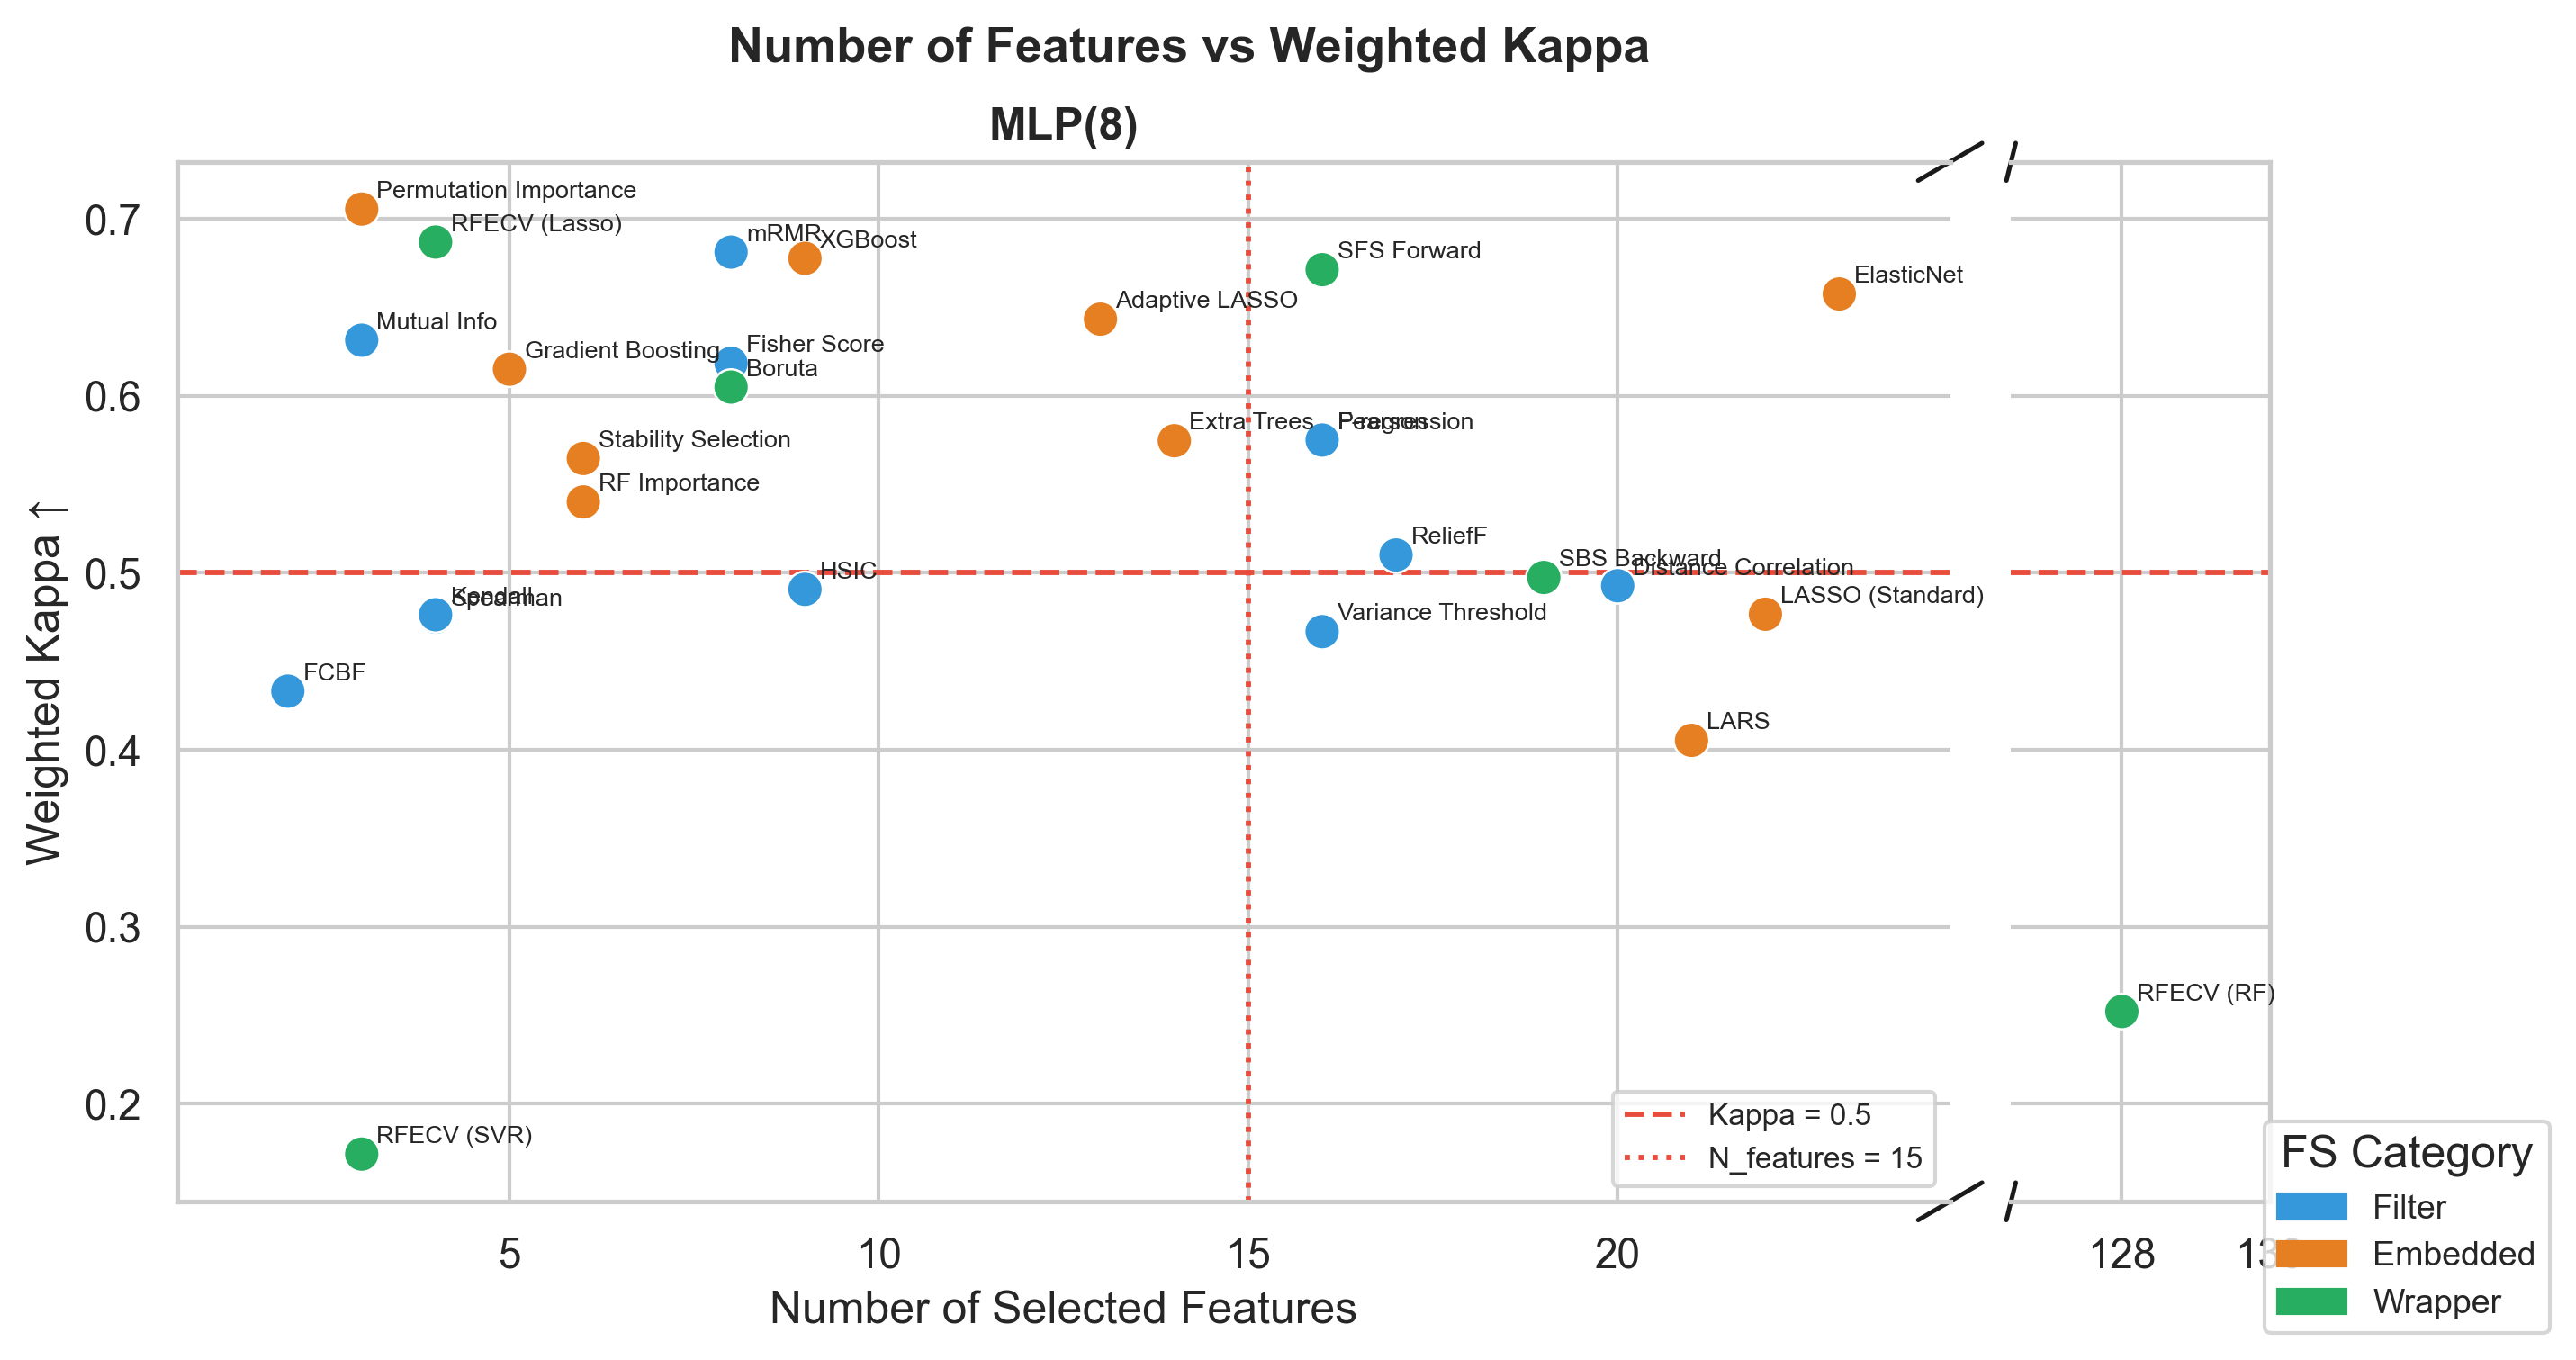
\includegraphics[width=0.85\textwidth,height=0.78\textheight,keepaspectratio]{figD_nfeats_vs_kappa.png}\\
    \scriptsize Red lines = Stage 5 filter (Kappa $\ge 0.5$, $N_\mathrm{feat} < 15$); \textbf{17/28} methods pass.
\end{frame}

%%%%%%%%%%%%%%%%%%%%%%%%%%%%%%%%%%%%%%%%%%%%%%%%%%%%%
\begin{frame}
    \frametitle{Feature Inclusion Frequency}
    \centering
    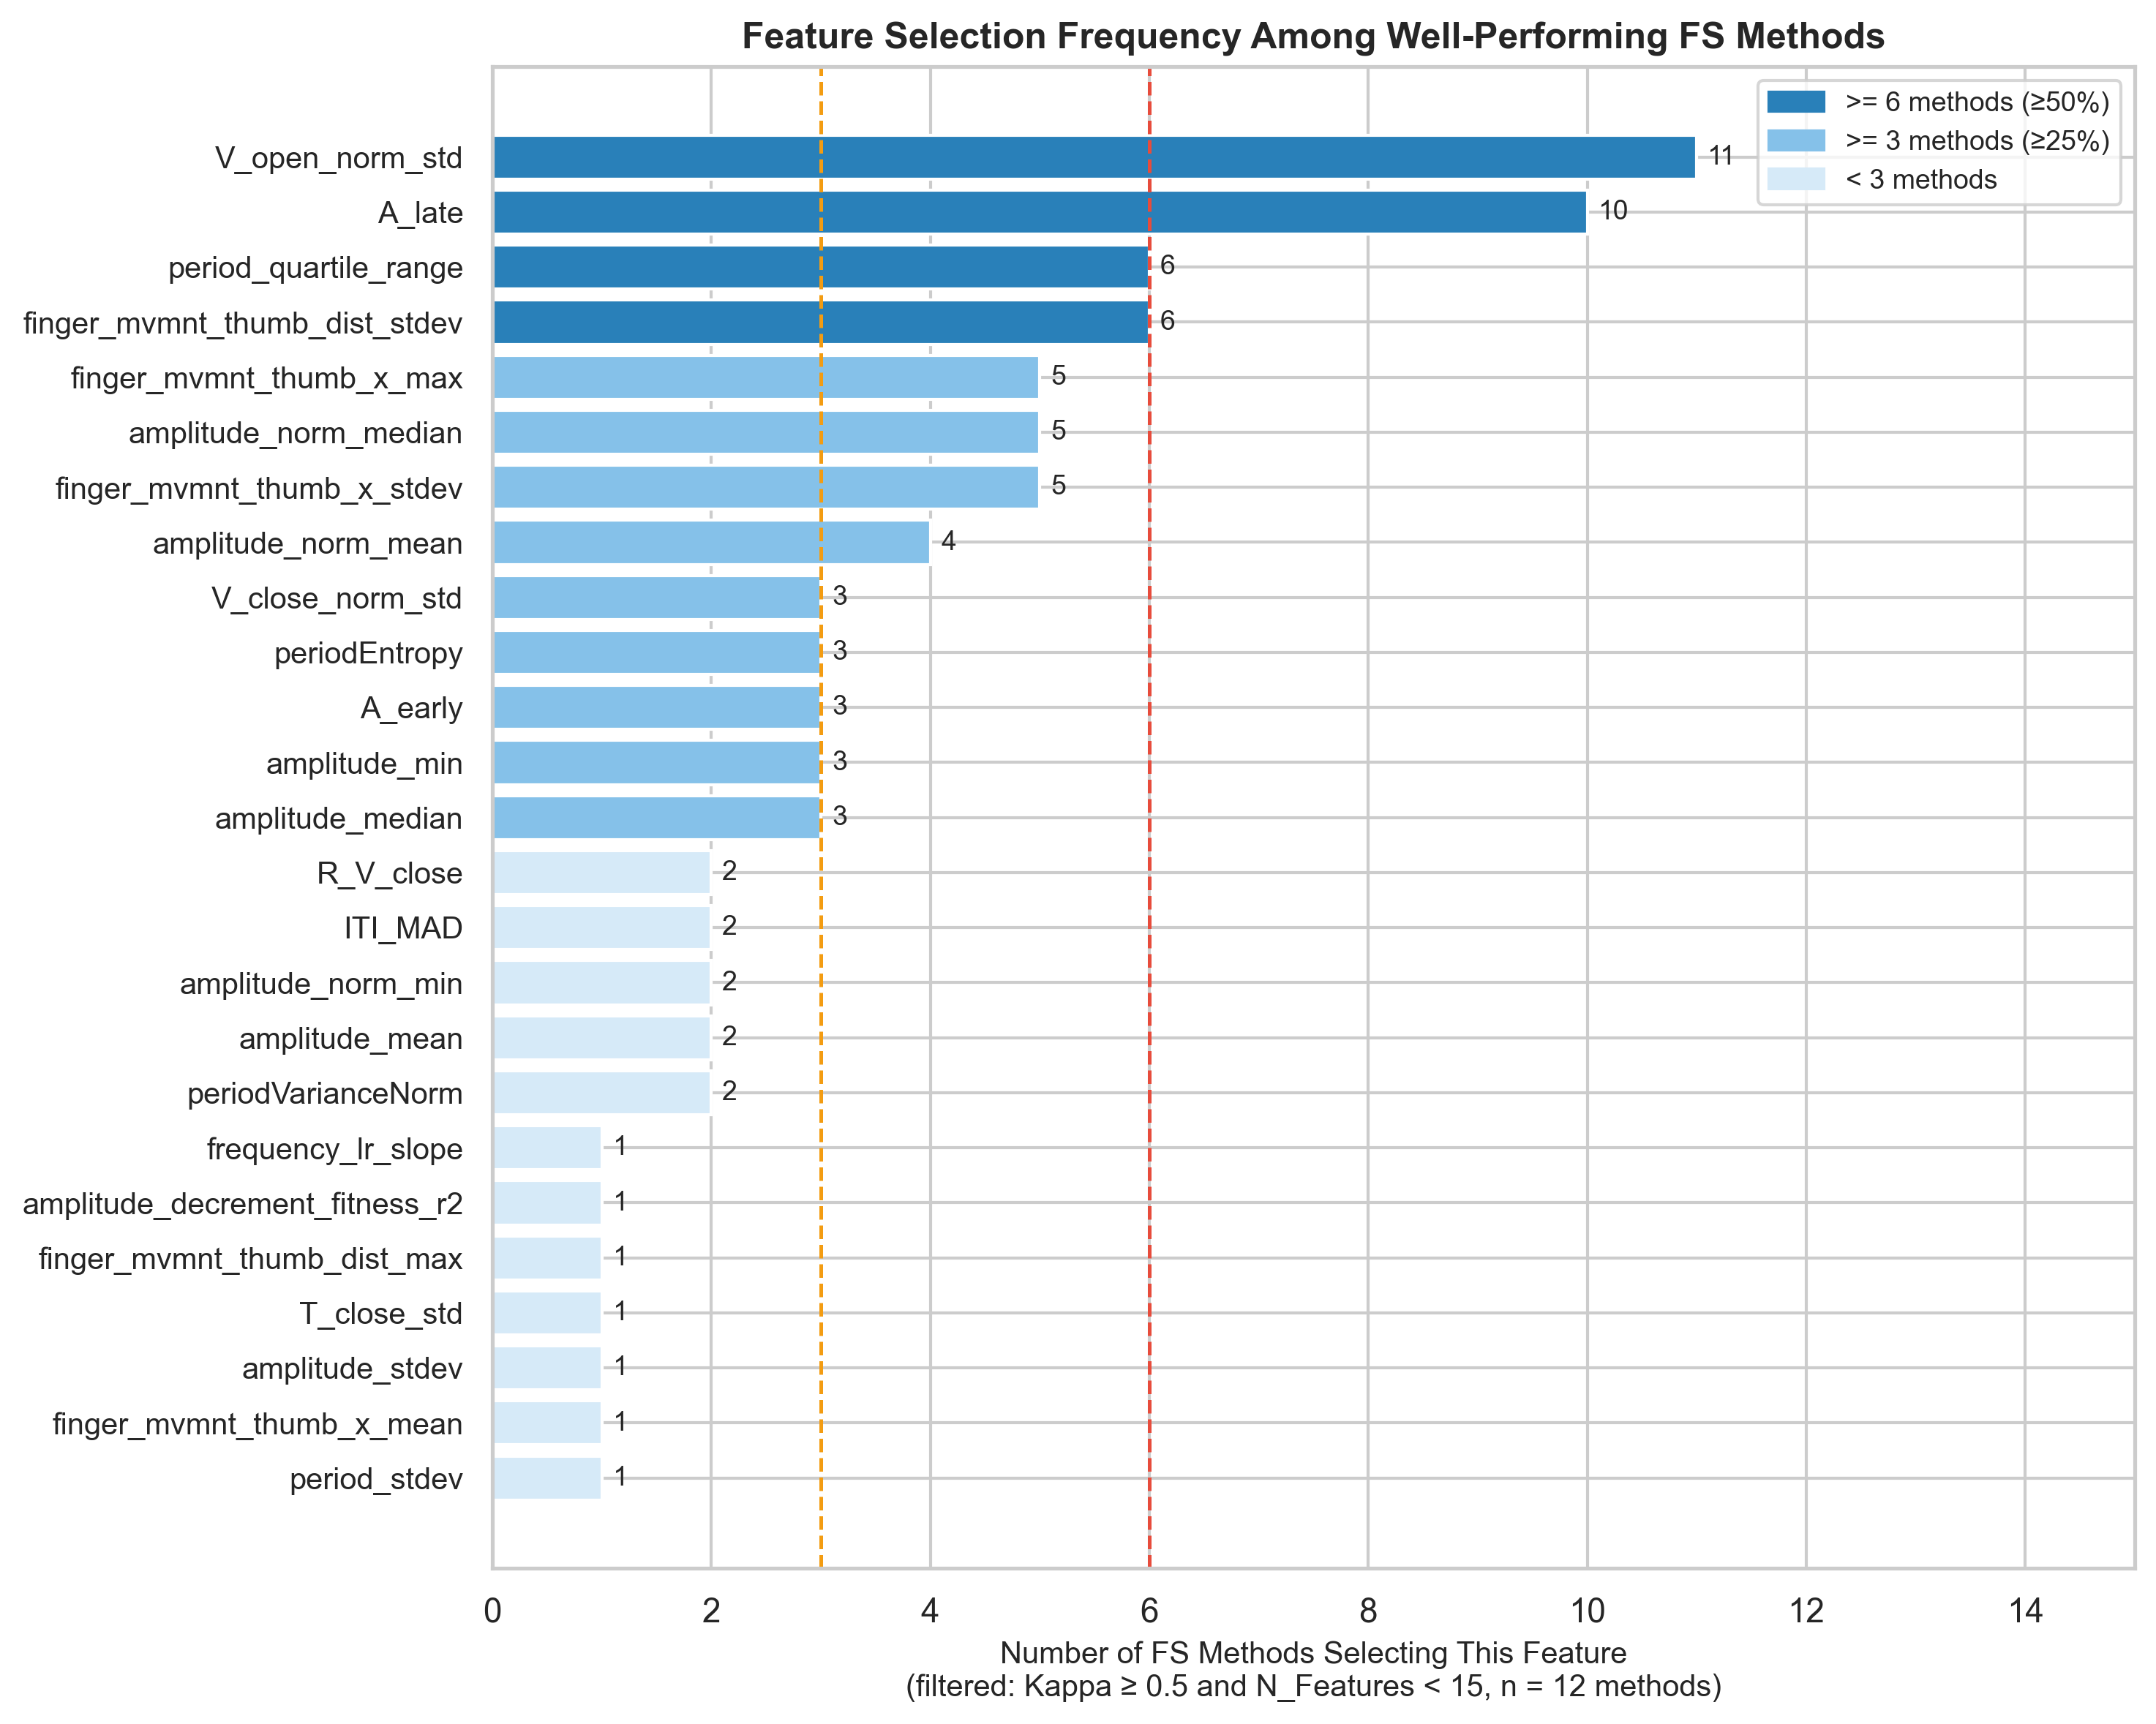
\includegraphics[width=0.62\textwidth,height=0.82\textheight,keepaspectratio]{figE_feature_frequency.png}\\
    \scriptsize Filter: only FS methods with Kappa $\ge 0.5$ AND $N_\mathrm{feat} < 15$ contribute (17 methods).
    Features picked by $\ge 50\%$ of these methods are strong candidates.
\end{frame}

%%%%%%%%%%%%%%%%%%%%%%%%%%%%%%%%%%%%%%%%%%%%%%%%%%%%%
%\begin{frame}
%    \frametitle{Top FS Methods (LOOCV, MLP-8, v2 features)}
%    \centering
%    \small
%    \begin{tabular}{lcccccc}
%        \toprule
%        FS Method & Category & $N$ & MAE $\downarrow$ & Spearman $\uparrow$ & Kappa $\uparrow$ & Composite \\
%        \midrule
%        Adaptive LASSO      & embedded & 8  & 0.340 & 0.736 & 0.741 & \textbf{0.937} \\
%        LASSO (Standard)    & embedded & 8  & 0.377 & 0.753 & 0.741 & 0.927 \\
%        LARS                & embedded & 8  & 0.377 & 0.753 & 0.741 & 0.927 \\
%        SBS Backward        & wrapper  & 8  & 0.302 & 0.783 & 0.738 & 0.872 \\
%        RF Importance       & embedded & 8  & 0.340 & 0.768 & 0.716 & 0.817 \\
%        RFECV (SVR)         & wrapper  & 6  & 0.340 & 0.719 & 0.720 & 0.780 \\
%        \midrule
%        RFECV (RF)          & wrapper  & 30 & 0.698 & 0.484 & 0.454 & 0.004 \\
%        \bottomrule
%    \end{tabular}
%    \\[0.4em]
%    \scriptsize Embedded \& wrapper methods dominate; RFECV\,(RF) fails due to overfitting on 30 features.
%\end{frame}

%%%%%%%%%%%%%%%%%%%%%%%%%%%%%%%%%%%%%%%%%%%%%%%%%%%%%
\begin{frame}
    \frametitle{Take-aways}
    \begin{itemize}
        \item \textbf{Embedded \& wrapper} methods dominate; pure-correlation filters underperform.
        \item \textbf{Adaptive LASSO, LASSO, LARS} achieve highest Kappa ($\approx 0.74$) with only 8 features.
        \item \textbf{SBS Backward} gives best Spearman (0.783) and MAE (0.302) -- most balanced.
        \item \textbf{RFECV (SVR)} is most compact: competitive Kappa (0.72) with only \textbf{6} features.
        \item 17/28 FS methods pass the Stage 5 filter; their frequency analysis gives a
              principled feature short-list for the LLM-Lasso prompt.
        \item Outputs in \texttt{fs\_results\_v2/\{png,pdf\}/}.
    \end{itemize}
\end{frame}

%%%%%%%%%%%%%%%%%%%%%%%%%%%%%%%%%%%%%%%%%%%%%%%%%%%%%
{
\setbeamertemplate{background}[NLTitle]
\setbeamertemplate{footline}[NLTitle]
\begin{frame}
    \begin{center}
        \vspace{1.5cm}
        {\Huge Thank you!}\\[0.6cm]
        {\large Questions \& Discussion}
    \end{center}
\end{frame}
}

\end{document}
